\documentclass[12pt]{beamer}

\def\languages{french, english}

%%%%%%%%%%%%%%%%%%% Theme

\usetheme{metropolis}

%%%%%%%%%%%%%%%%%%% Libraries

%%%%%%%%%% Packages

\usepackage[
backend=biber,
style=numeric-comp,
sorting=none,
maxbibnames=99
]{biblatex}
%%%%%%%%%% Packages

%%%%% Coding tools

\usepackage{comment}
\usepackage{xstring}

%%%%% Encoding

\usepackage[utf8]{inputenc}
\usepackage[T1]{fontenc}
\usepackage{eurosym}

%%%%% Languages

\ifx\languages\undefined
	\usepackage[english]{babel}
\else
	\usepackage[\languages]{babel}
\fi

\def\languagefile{./include/languages/\languagename.tex}
\InputIfFileExists{\languagefile}{}

%%%%% Style

\usepackage{csquotes}
\usepackage{color}
\usepackage{textpos}

\newcommand\titlelogo[1]{
	\titlegraphic{
		\hfill\includegraphics[height=0.2\textheight]{#1}
	}
}

\newcommand\framelogo[1]{
	\addtobeamertemplate{frametitle}{}{
		\begin{textblock*}{\textwidth}(\textwidth,-1.28\baselineskip)
			\includegraphics[height=\baselineskip]{#1}
		\end{textblock*}
	}
}

%%%%%%%%%% Packages

\usepackage{float}
\usepackage[skip=1em]{caption}

\usepackage{array}
\usepackage{multirow}
\usepackage{multicol}

%%%%%%%%%% Features

%%%%% Settings

\renewcommand{\arraystretch}{1.2}

%%%%% Commands

\newcommand\noskipcaption[1]{\caption{#1}\vspace{-1em}}
\newcommand\noskipcaptionstar[1]{\caption*{#1}\vspace{-1em}}

%%%%%%%%%% Packages

\usepackage{siunitx}

%%%%%%%%%% Features

%%%%% Settings

\ifx\decimalsign\undefined
\else
    \sisetup{output-decimal-marker = \decimalsign}
\fi


%%%%%%%%%%%%%%%%%%% Bibliography

\addbibresource{resources/bib/sample.bib}

%%%%%%%%%%%%%%%%%%% Titlepage

\title{Renewable Energy Production Forecast}
\subtitle{PROJ0016 - Big Data Project}
\author{Yann Claes, Gaspard Lambrechts and François Rozet}
\institute{University of Liège}
\date{\today}
\titlelogo{resources/pdf/logo.pdf}
\framelogo{resources/pdf/logo.pdf}

%%%%%%%%%%%%%%%%%%%

\begin{document}

\maketitle

\begin{frame}{Road Map}
    \begin{figure}
        \centering
        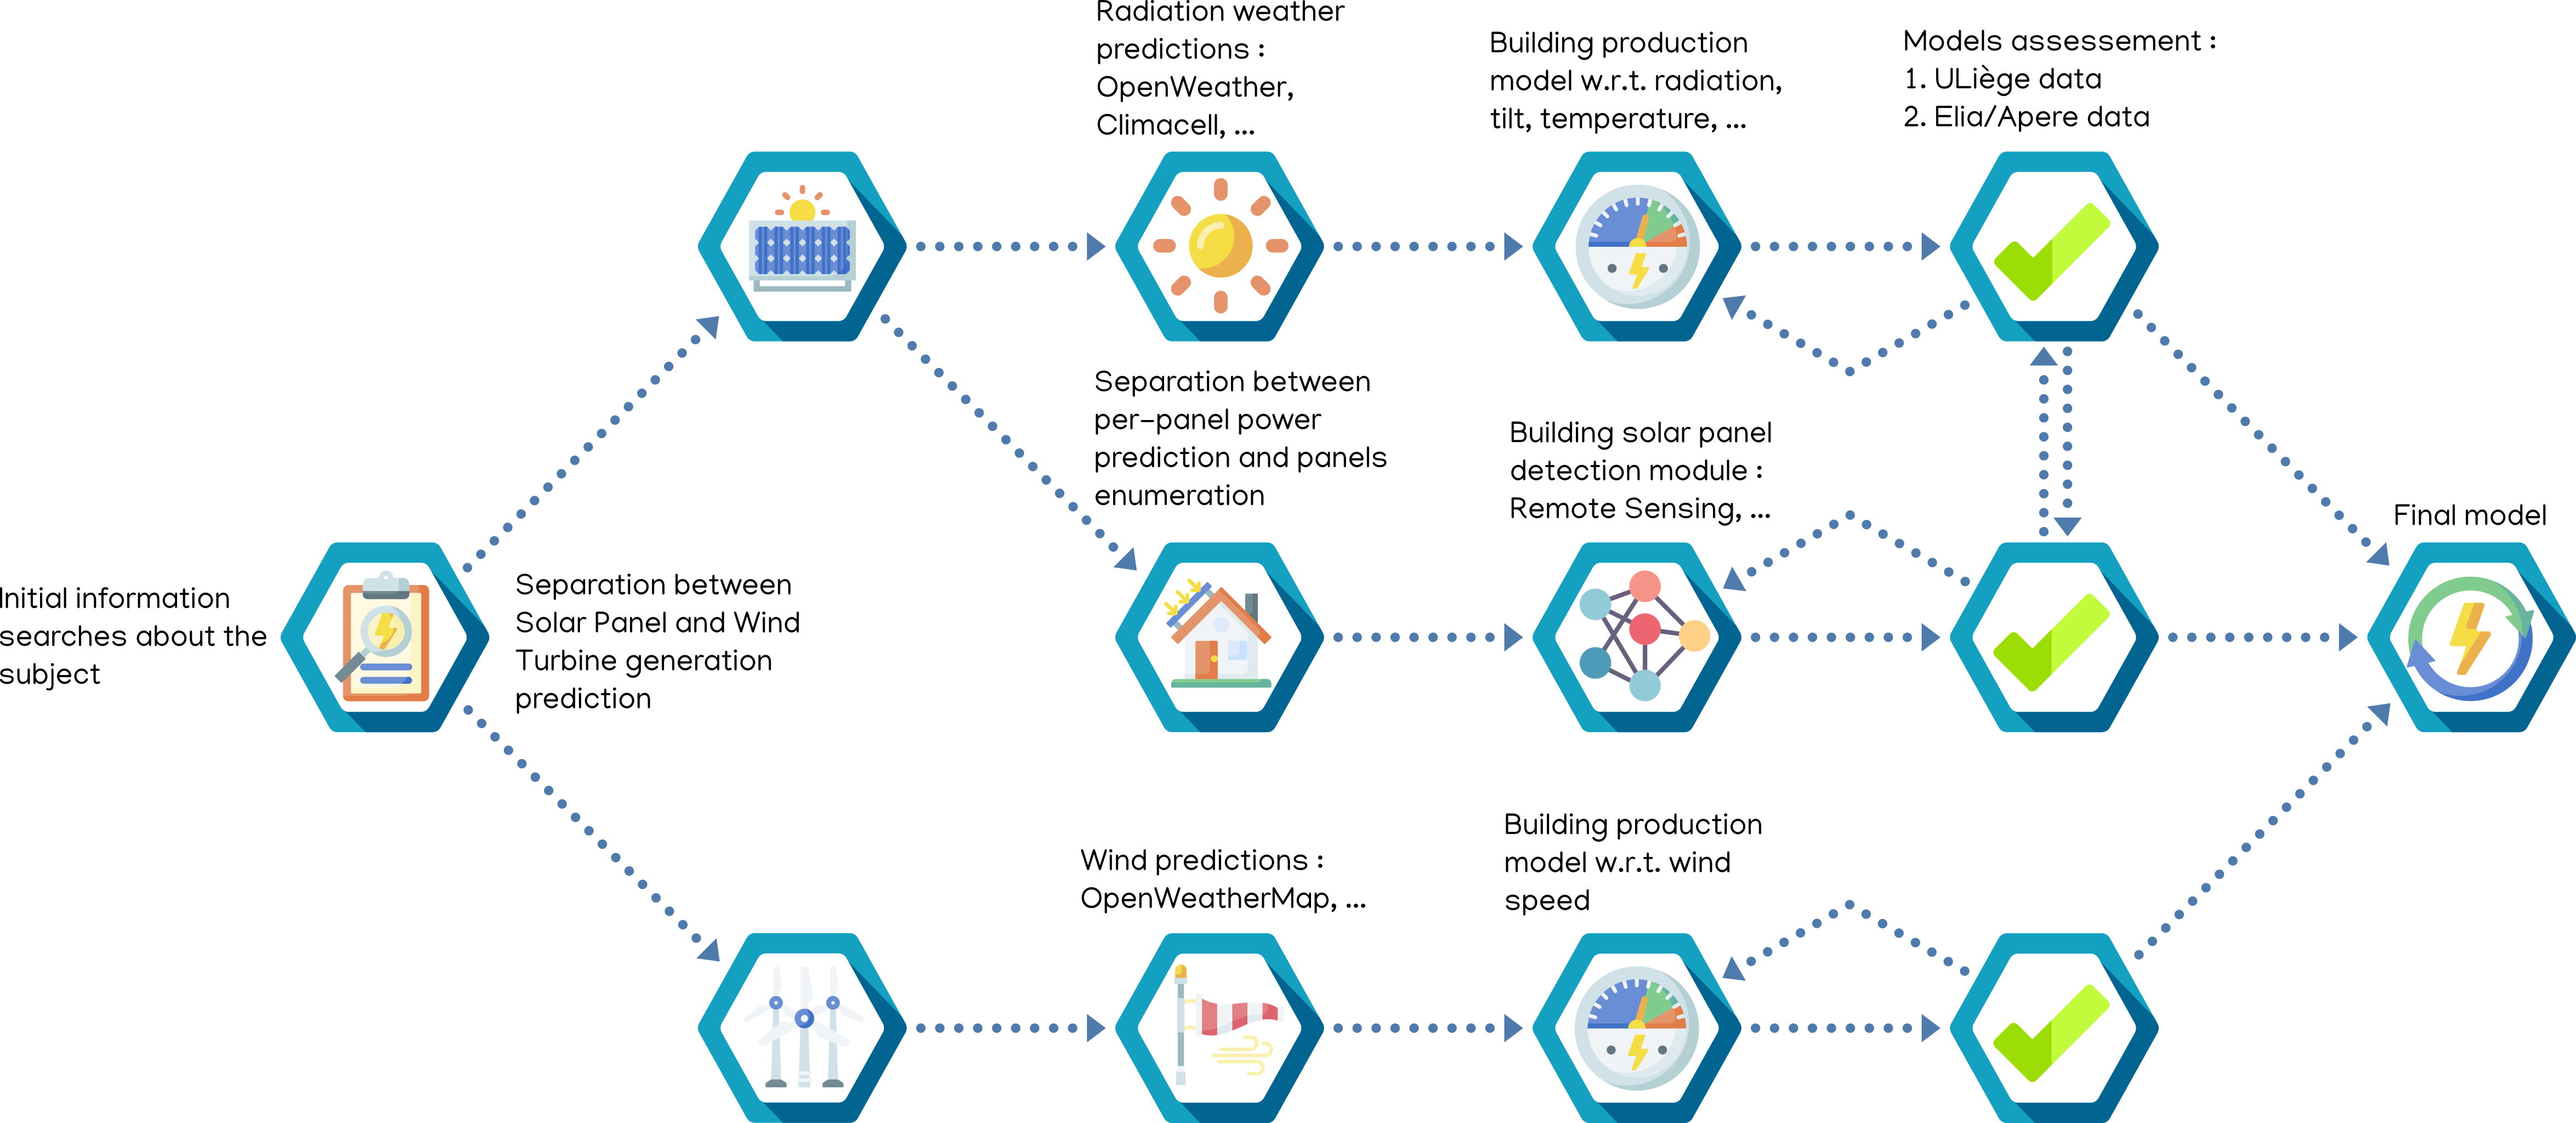
\includegraphics[width=\textwidth]{resources/png/roadmap.png}
    \end{figure}
\end{frame}

\section{Photovoltaic Production}

\begin{frame}{Influencing Parameters}
    \begin{itemize}
        \item \alert{Tilt} $\beta$ of the panel
        \item \alert{Surface azimuth} $A_s$ of the panel
        \item Module \alert{efficiency} $\eta$
        \item Module \alert{area} $A$
    \end{itemize}
\end{frame}

\begin{frame}{Influencing Parameters}
    \begin{itemize}
        \item \alert{Temperature} $T$
        \item \alert{Irradiance} received by the panel $I$
        \item \alert{Incidence angle} $\theta$ between the sun rays and the normal to the panel
    \end{itemize}
\end{frame}

\begin{frame}{Resulting Model}
    Combining these parameters yielded the following model:
    
    \begin{equation*}
        P_{out} = \eta I \cos(\theta) A
    \end{equation*}
    
    which gives the output power of the photovoltaic panel in Watts (bounded by $P_{max}$, the maximum output power of the panel).
\end{frame}

\begin{frame}{Incidence Angle}
    The cosine of the incidence angle can be expressed as\cite{itaca}:
    
    $$
    \begin{aligned}
        \cos(\theta) & = \sin(\delta)\sin(\phi)\cos(\beta) + \sin(\delta)\cos(\phi)\sin(\beta)\cos(A_s) \\
        & + \cos(\delta)\cos(\phi)\cos(\beta)\cos(\omega) \\
        &- \cos(\delta)\sin(\phi)\sin(\beta)\cos(A_s)\cos(\omega) \\
        &-  \cos(\delta)\sin(\beta)\sin(A_s)\sin(\omega)
    \end{aligned}
    $$
    
    where solar angles can be computed using \alert{pvlib}.
\end{frame}

\begin{frame}{Challenges}
    \begin{itemize}
        \item Panel \alert{type} evaluation
        \item Module \alert{efficiency} evaluation
        \item Module maximum power \alert{$P_{max}$} evaluation
        \item Panel \alert{tilt} evaluation
        \item Finding irradiance \alert{forecast} data
    \end{itemize}
\end{frame}

\begin{frame}{Example Model}
    An example model has been implemented on the Sart-Tilman data (using the thermodynamics laboratory data).
\end{frame}

\begin{frame}{Example Model}
    \begin{figure}
        \centering
        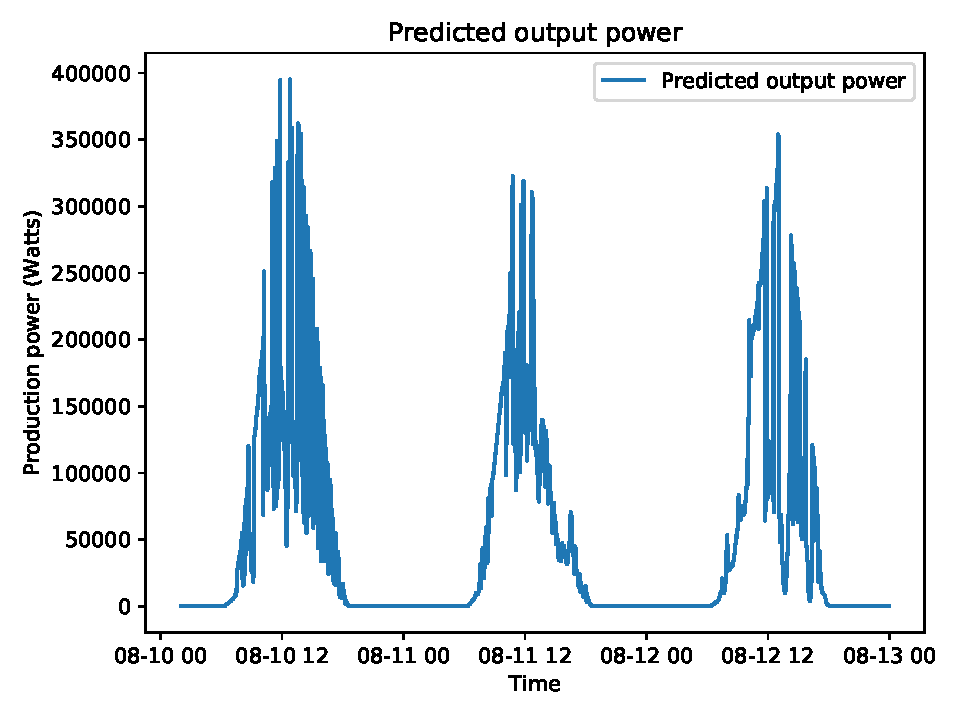
\includegraphics[width=0.9\textwidth]{resources/pdf/predicted_power.pdf}
    \end{figure}
\end{frame}

\begin{frame}{Example Model}
    \begin{figure}
        \centering
        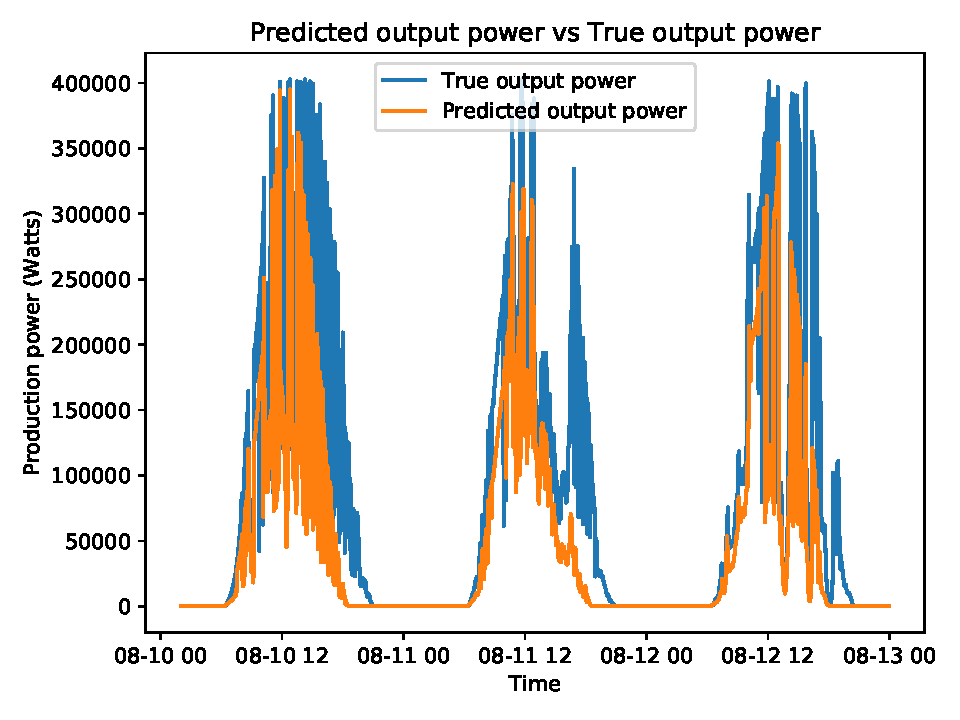
\includegraphics[width=0.9\textwidth]{resources/pdf/predicted_vs_true.pdf}
    \end{figure}
\end{frame}

\begin{frame}{Next objectives}
    \begin{itemize}
        \item Maximum power \alert{bounding}
        \item \alert{Temperature} influence
        \item Potential \alert{scaling} of the irradiance
    \end{itemize}
\end{frame}

\section{Photovoltaic panels enumeration}

\begin{frame}{Test set -- WalOnMap}
    Wallonia possesses a \texttt{WebMapService} : \alert{WalOnMap}.
    
    It gives access to high quality (\SI{1}{px} per \SI{25}{\centi\meter}) georeferenced images of the region\footnote{The satellite pictures were taken in \alert{2018}.}.
\end{frame}

\begin{frame}{Test set -- WalOnMap}
    Based on \alert{WalOnMap} API, we have produced a \alert{prototype} python program to retrieve an image w.r.t. some geo-localisation.
    \begin{center}
        \texttt{\$ python3 wms.py 50.637082 5.564001 50}
    \end{center}
\end{frame}

\begin{frame}{Test set -- WalOnMap}    
    \begin{figure}
        \centering
        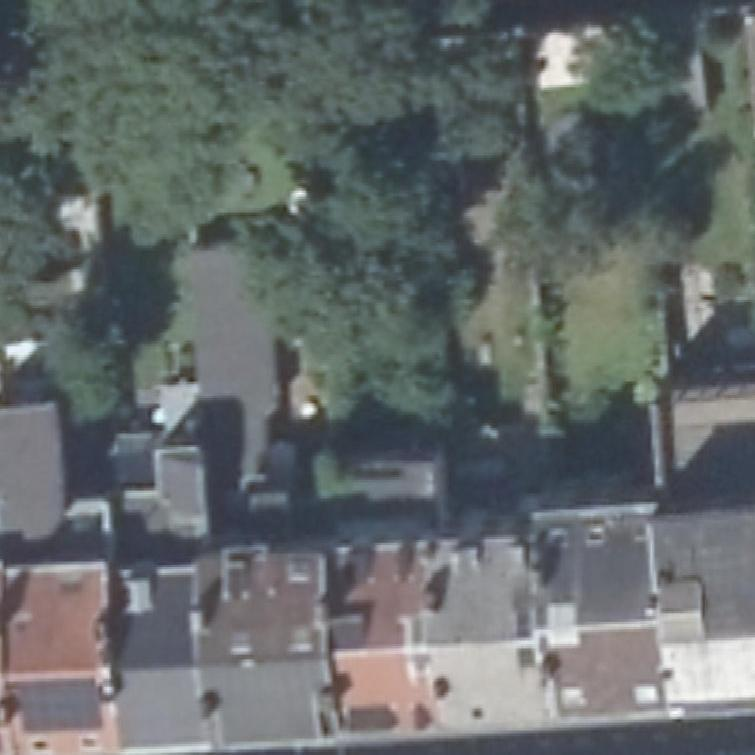
\includegraphics[width=0.70\textwidth]{resources/png/walonmap.jpg}
    \end{figure}
\end{frame}

\begin{frame}{Test set -- GoogleMaps}    
    There is also an API for \alert{GoogleMaps}.
    
    Google Maps has an even finer resolution and more recent satellite pictures.
    
    We will try to obtain an API \alert{key}.
\end{frame}

\begin{frame}{Test set -- GoogleMaps}
    \begin{figure}
        \centering
        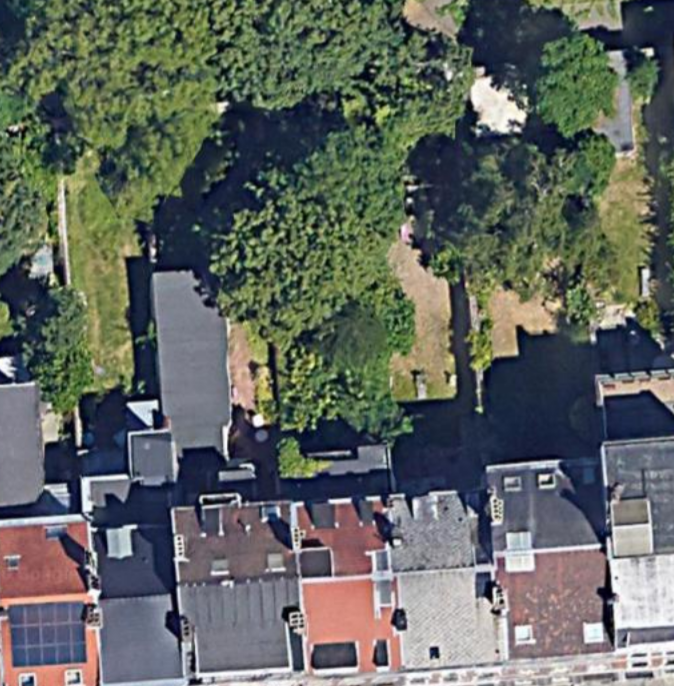
\includegraphics[width=0.70\textwidth]{resources/png/googlemaps.png}
    \end{figure}
\end{frame}

\begin{frame}{Detection model -- DeepSolar}
    \begin{itemize}
        \item The network isn't provided pre-trained
        \item The learning set isn't publicly available
        \item Written in \texttt{Python 2.7} (Deprecated)
    \end{itemize}
    We need another solution.
\end{frame}

\begin{frame}{Detection model}
    We found some alternatives :
    \begin{itemize}
        \item DeepSolaris (BISS Institute, Heerlen)
        \item Solar Panel Detection (Alan Turing Institute)
        \item Automatic solar photovoltaic panel detection in satellite imagery (Duke University)
        \item ...
    \end{itemize}
    Interesting methods \alert{but} no trained model or training data.

    We \alert{need} training data.
\end{frame}

\begin{frame}{Training data}
    Two ideas :
    \begin{enumerate}
        \item Annotating (by hand) satellite pictures with/without solar panels\footnote{For example using \alert{Cytomine}.}. Total control but dummy work. Also, we still need to know \emph{some} panel coordinates.
        \item Finding (or asking for) a solar panel coordinates dataset.
        
        We have one for England (\alert{OpenStreetMap}), but it is very imprecise and only gives a \alert{position}. Problem : we need a \alert{surface} for training a segmentation network.
    \end{enumerate}
\end{frame}

\begin{frame}{Training data}
    \begin{figure}
        \centering
        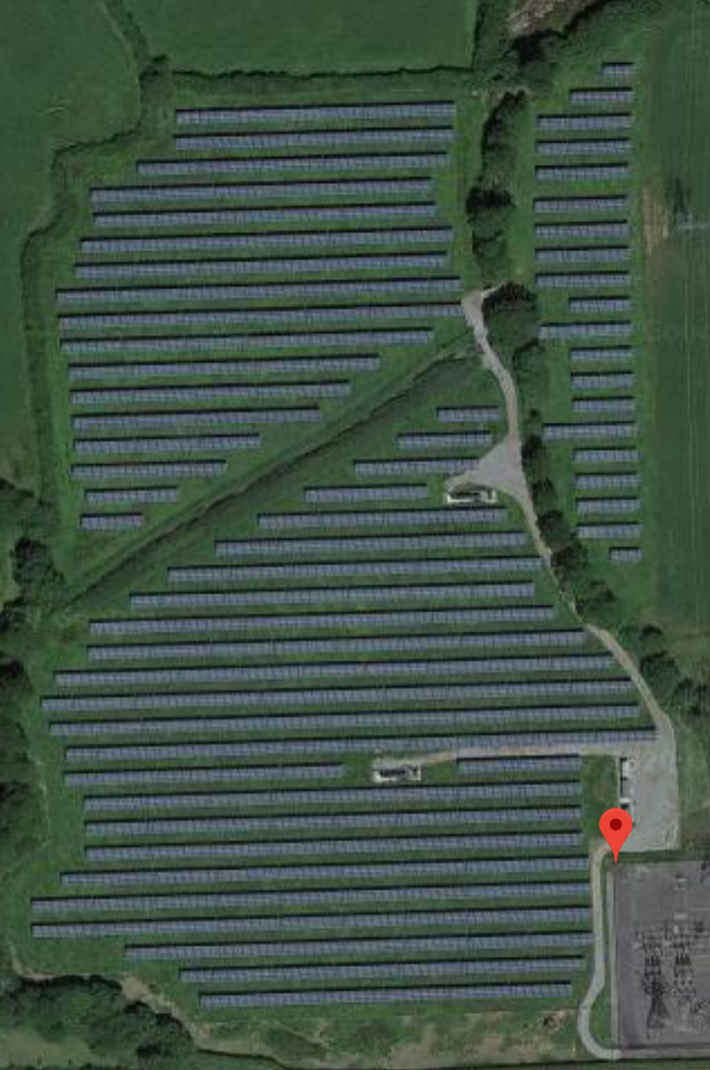
\includegraphics[width=0.5\textwidth]{resources/png/england.png}
    \end{figure}
\end{frame}

\begin{frame}{Next objectives}
    Short term
    \begin{itemize}
        \item Find quickly a suitable training set.
        \item Maybe build a simple computer vision detection model.
    \end{itemize}
    Long term
    \begin{itemize}
        \item Surface, orientation and (maybe) tilt detection.
    \end{itemize}
\end{frame}

\section{Wind Power Production}

\begin{frame}{Wind turbines enumeration}
    \begin{itemize}
        \item SPW Energie data (2018)
    \end{itemize}
    \begin{figure}
        \centering
        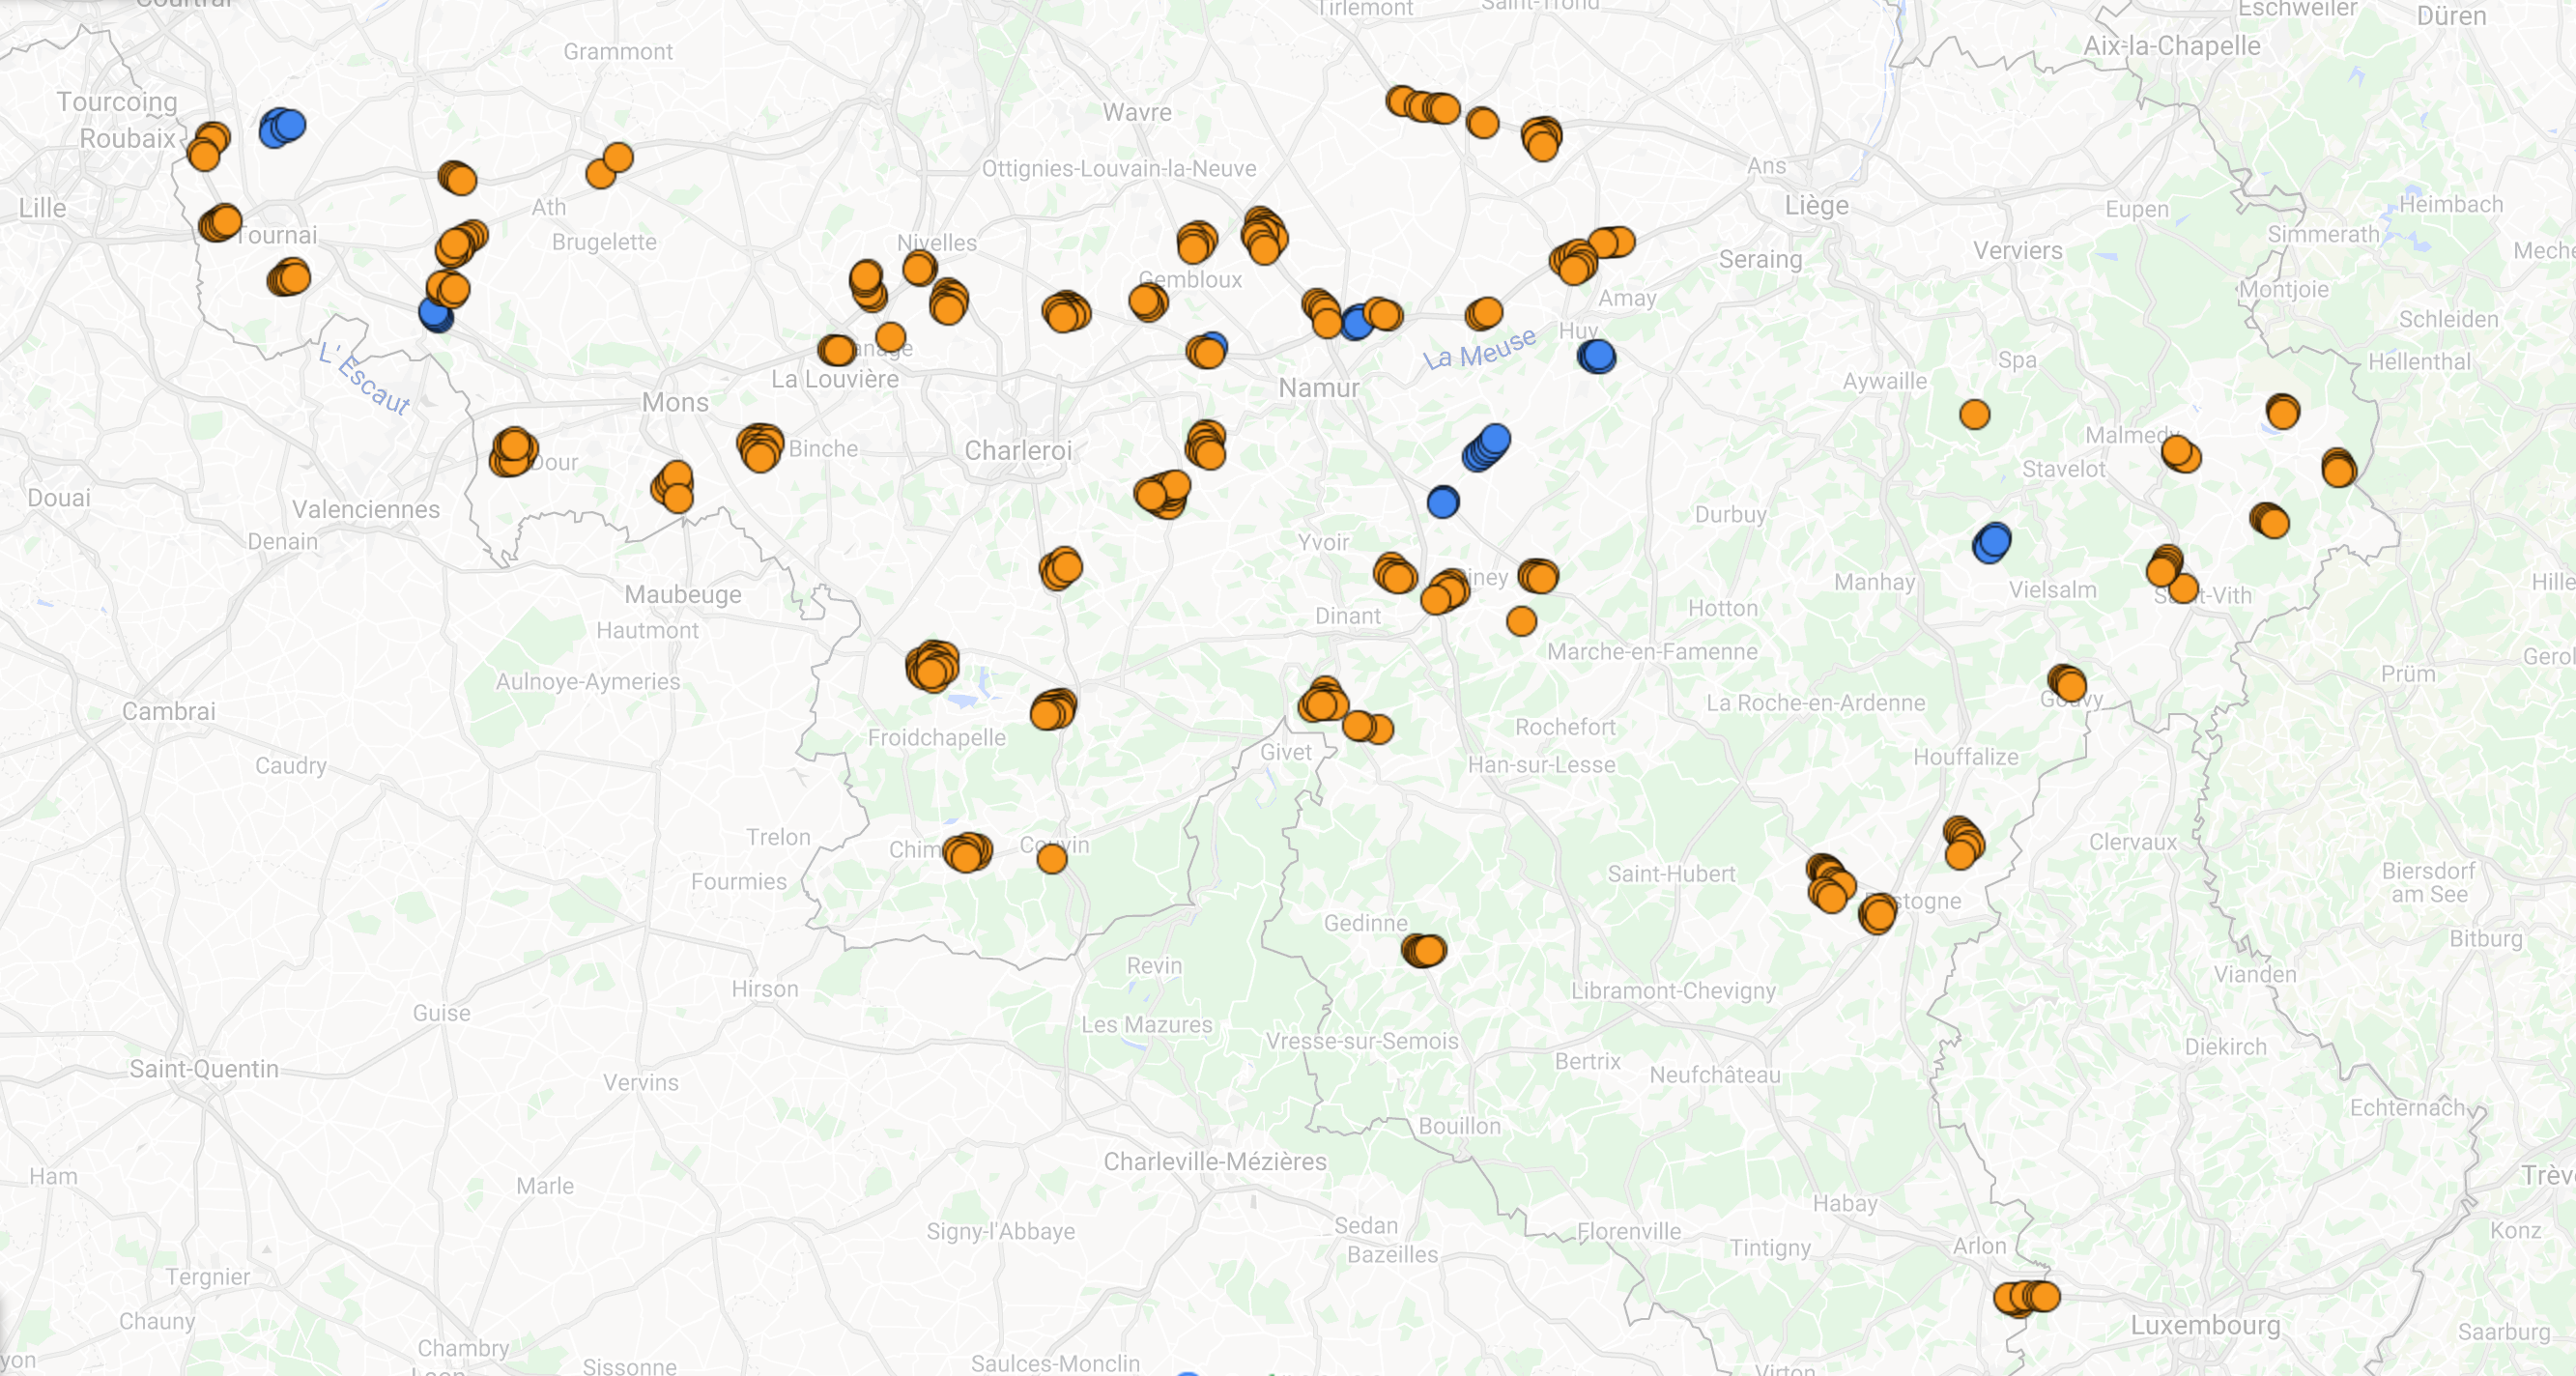
\includegraphics[width=0.9\textwidth]{resources/png/SPW_data.png}
        \caption*{SPW Energie - Wind turbines map \cite{spwe-wind-turbines}}
    \end{figure}
\end{frame}

\begin{frame}{Wind turbines enumeration}
    \begin{itemize}
        \item Outdated (+13.97\% MWp in 2019 in Wallonia: 127MW)
    \end{itemize}
    \begin{figure}
        \centering
        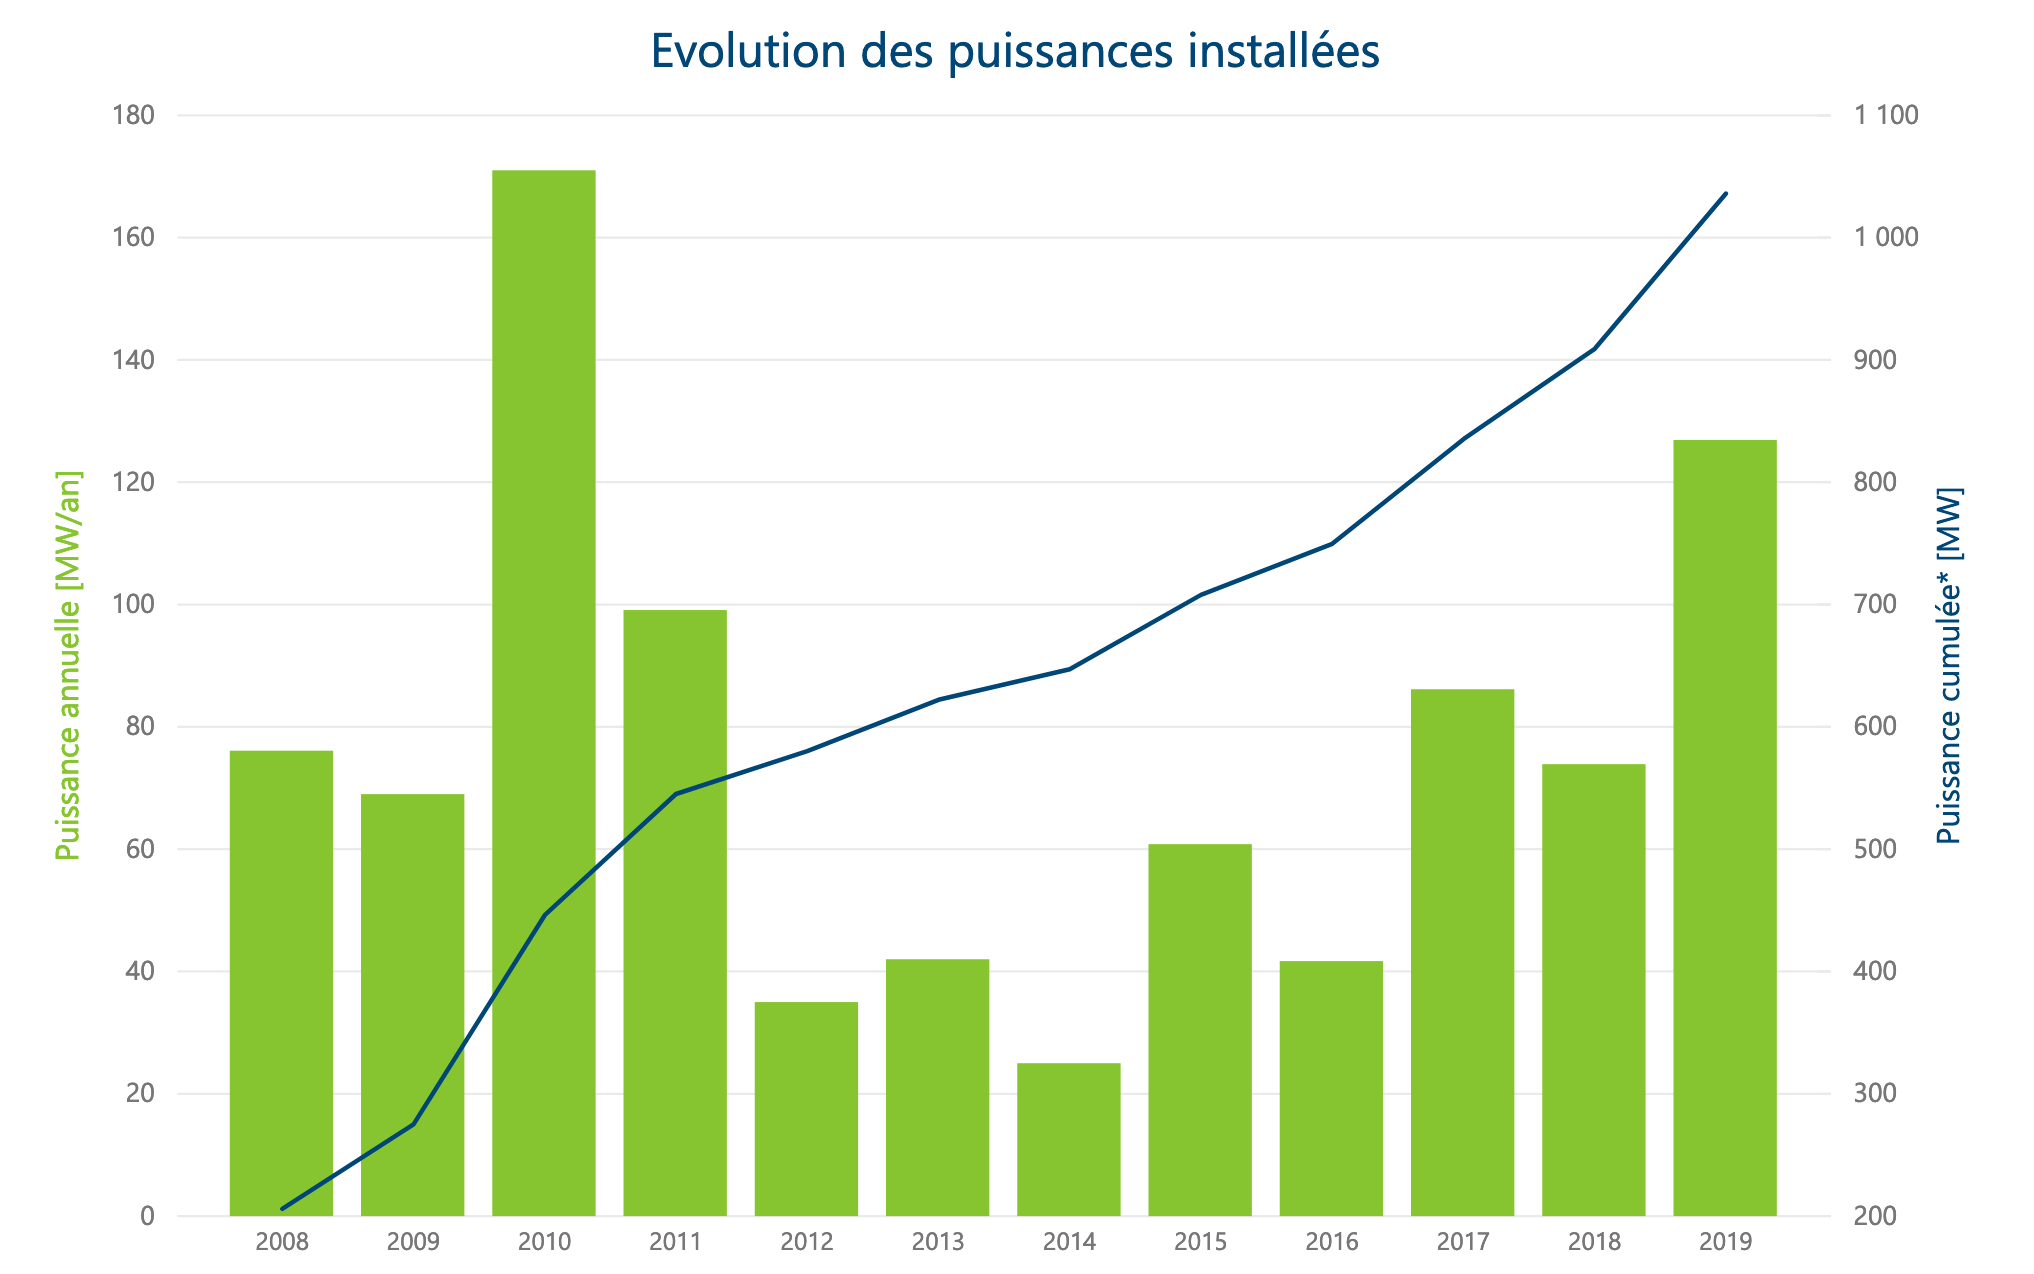
\includegraphics[width=0.9\textwidth]{resources/png/APERe_total_power.png}
        \caption*{APERe - Wind power in Wallonia \cite{elia_wind}}
    \end{figure}
\end{frame}

\begin{frame}{Wind turbines characteristics}
    \begin{itemize}
        \item Metadata of the KML Google Maps file from the SPW Energie (one row for each unique wind turbine in Wallonia):
            \resizebox{\linewidth}{!}{
            \begin{tabular}{|c|c|c|c|c|c|c|c|c|c|}
                \hline
                Id&CodeCWaPE&Exploitant&Localisation&\color{red}{Puissance}&\color{blue}{Lat}&\color{blue}{Long}&\color{red}{Marque}&\color{red}{Type}&Etat\\
                \hline
            \end{tabular}
        }
    
        \item Each unique \texttt{(Marque, Type, Puissance)} is extracted.
        
        \item \alert{Model of power production} w.r.t the \alert{wind} for each of these unique tuple.
        
        \item Need of \alert{power curve} data for each of these models
    \end{itemize}
\end{frame}

\begin{frame}{Wind turbines characteristics - Power curves}
    Data from website \textit{Wind Turbines Models} \cite{wind-turbine-models} includes:
    \begin{itemize}
        \item Cut-in, cut-out, rated wind speed
        \item Hub height
        \item (Most of the time) a 20-50 data-points discrete power curve
    \end{itemize}
    \begin{figure}
        \centering
        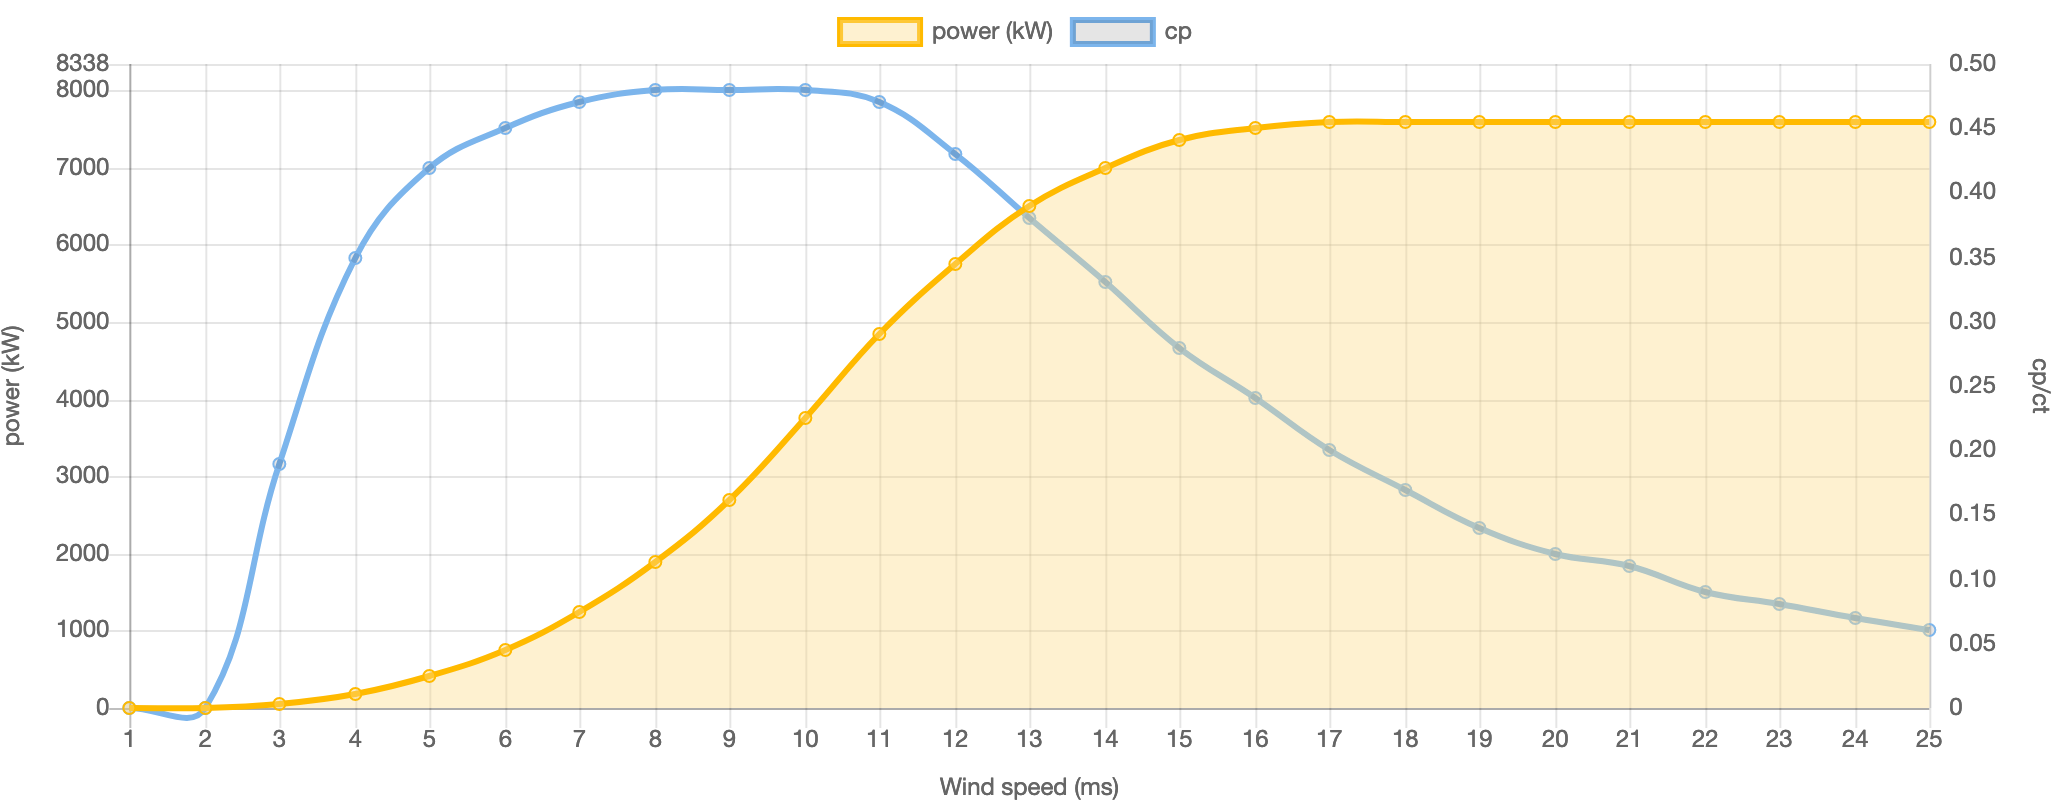
\includegraphics[width=.5\textwidth]{resources/png/power_curve.png}
        \caption*{Enercon E-126 Power Curve}
        \label{fig:my_label}
    \end{figure}
\end{frame}

\begin{frame}{Wind turbines characteristics - Models}

According to the availability of the power curve, the model built for a certain \texttt{(Marque, Type, Puissance)} is : 
\begin{itemize}
    \item {a \alert{cubic spline interpolation of the power curve data}} between the cut-in and cut-out wind speed, or
    \item a \alert{naive theoretical model} where the power:
    \begin{itemize}
        \item is 0 between 0 and the cut-in wind speed
        \item is 0 above the cut-out wind speed
        \item is the peak power of the wind turbine between the rated and the cut-out wind speed
        \item is proportional to the cubed wind speed between the cut-in and rated wind speed, as the theoretical wind power is $\frac{1}{2} \eta \rho A v^3$.
    \end{itemize}
\end{itemize}
    
\end{frame}

\begin{frame}{Weather}
    For now, we use free weather API that provides limited information:
    
    \resizebox{\textwidth}{!}{
        \begin{tabular}{|c|c|c|c|c|c|}
            \hline
            API & Live & Nowcast & Forecast & Solar Radiation & History\\
            \hline
            OpenWeatherMap & x & - & 3h (5d) & - & - \\
            \hline
            Climacell & x & 5min (5h) & 1h (5d) & x & - (?) \\
            \hline
            Darksky & x & 1min (1h) & 1h (1d) & - & x \\
            \hline
        \end{tabular}
    }
    
\end{frame}

\begin{frame}{Aggregated Wind Power Production}
    Whereas the final model should only focus on the Liege province, here we consider all wind turbines of Wallonia, in order to compare with \alert{Elia's mmeasures}
    
    For \alert{each wind turbines}, 
    \begin{itemize}
        \item Weather API query in order to get the \alert{wind speed} at this location (lat, lon)
        \item Power production estimated thanks to the wind and the \texttt{(Marque, Type, Puissance)} \alert{model}.
    \end{itemize}
    
    Then, all individual powers are summed up.
\end{frame}

\begin{frame}{Results}
    Running a quick model \alert{using only the wind speed at Liege} yielded the following results for the \alert{last three days}:
    \begin{figure}
        \centering
        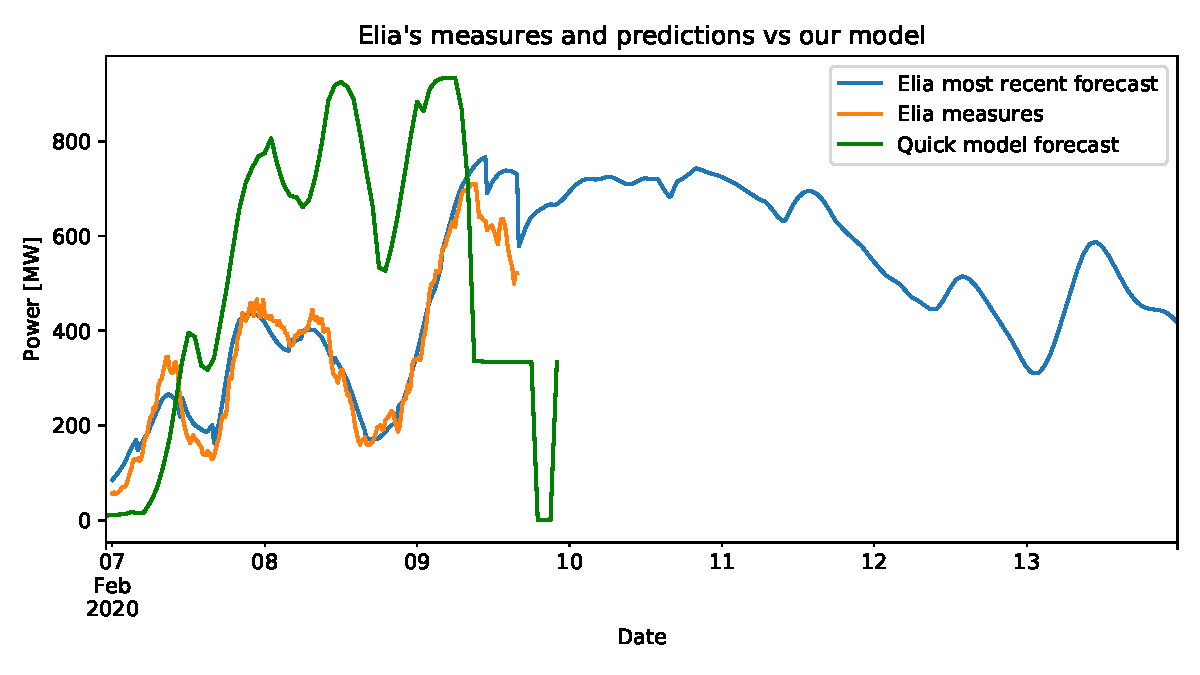
\includegraphics[width=\textwidth]{resources/pdf/quick_model_liege.pdf}
    \end{figure}
\end{frame}

\begin{frame}{Results}
    Running a quick model \alert{using the wind speed at each power plant} yielded the following results for the \alert{last three days}:
    \begin{figure}
        \centering
        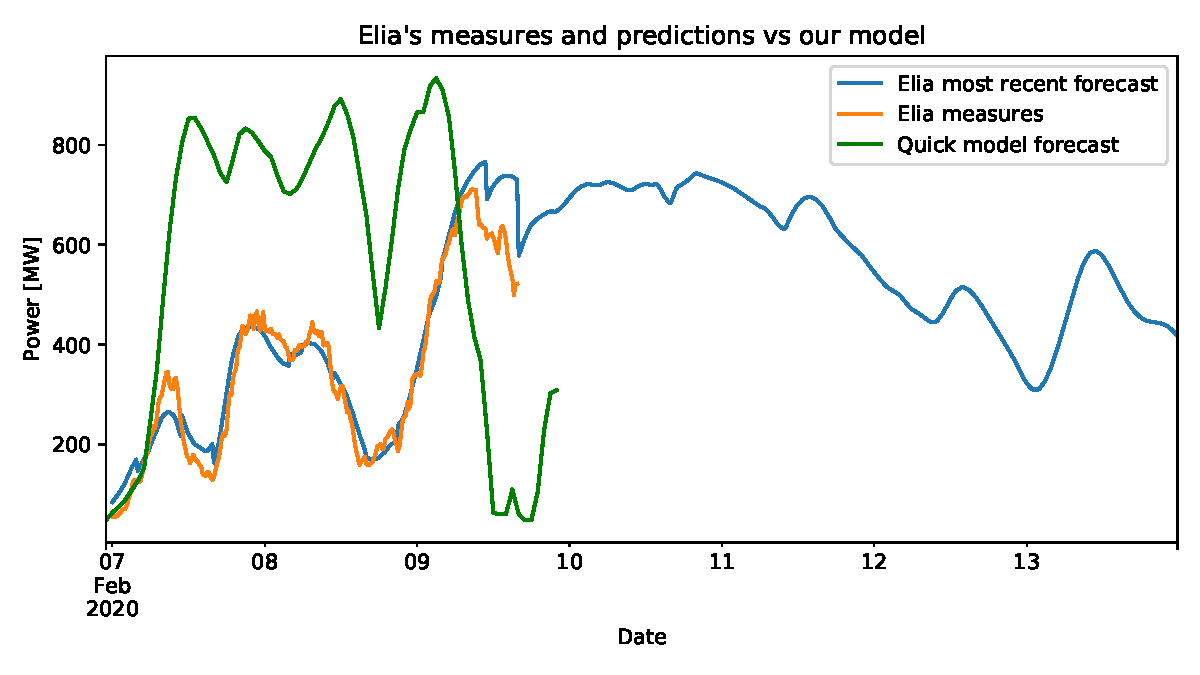
\includegraphics[width=\textwidth]{resources/pdf/quick_model.pdf}
    \end{figure}
\end{frame}

\begin{frame}{Next objectives}
    \begin{itemize}
        \item Getting a \alert{more recent list of wind turbines}
        \item Getting a \alert{power curve} for each existing type of wind turbine in Wallonia
        \item Using the \alert{hub height} to get a more precise wind speed at rotor height
        \item \alert{Understanding the gap} between Elia's prediction and ours
        \item Getting hourly power production data from some wind turbines to \alert{identify where the differences come from}.
    \end{itemize}
\end{frame}

\begin{frame}[allowframebreaks]
    \printbibliography
\end{frame}

\end{document}
